\chapter{Teoretyczne podwaliny}
\label{chap:teoretyczne_podwaliny}

Treść dla rozdziału pierwszego zwykle zawiera w sobie teoretyczne podwaliny pod dalszą część Twojej pracy dyplomowej (czy to licencjackiej, magisterskiej lub nawet doktorskiej).

Jak również zapewne zauważyłeś drogi Czytelniku, rozdział ten posiada już normalną numerację, tak jak to powinno wyglądać w wydruku dla pracy końcowej (patrz spis treści).

\begin{table}[!h]
    \centering
    \begin{tabular}{|c|c|}
    \hline
    \textbf{Kolumna 1} & \textbf{Kolumna 2} \\ \hline \hline
    wiersz1-kolumna1 & wiersz1-kolumna2 \\ \hline
    wiersz2-kolumna1 & wiersz2-kolumna2 \\ \hline
    \end{tabular}
\caption{Prosta tabelka dla przykładu}
\label{tab:tab:prosta-tabela-przyklad-A}
\end{table}


\section{Przykładowy podrozdział 1-go rzędu}
Jak widać można zagnieżdżać treści w wygodne sekcje (ang. \textit{sections}) tak jak również w~dowolnym momencie umieszczać rysunki lub fotografie --- tak jak to widać na rysunku~\ref{fig:word-vs-latex}.

\begin{figure}[!ht]
\centering
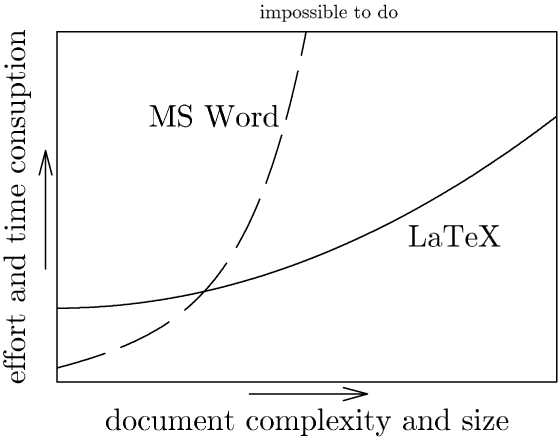
\includegraphics[width=100mm]{images/word-vs-latex.png}
\captionsource{Trudnośc pisania dokumentów w stosunku do ich objętości}{\url{http://www.pinteric.com/miktex.html}}
\label{fig:word-vs-latex}
\end{figure}

Czasem zdaży się również tak, że przeniesie zdjęcie na kolejną stronę, jednak w~pewnych okolicznościach to celowy zabieg który wykonuje za nas kompilator LaTeXa --- Super! :) \\
Wtedy można bez kołototu odwołać się do konkretnego zdjęcia, tabeli, kodu źródłowego, przypisu bibliograficznego, ect. poprzez referecję (komendę \texttt{\textbackslash{}ref\{?\}} i podanie zamiast znaku zapytania odwołania, czyli tzw. \texttt{label}-ki). Całość opisaną powyżej mozna odnaleźć w kodzie źródłowym do niniejszego rozdziału. Tak, to na prawdę jest, aż takie proste :)

\subsection{Podrozdział 2-go rzędu}
\label{subsec:podrozdzial-2-rzedu}

A tu przykład kolejnego zagnieżdzenia. Zwylke wystarczają 2 w 3 stopniowej skali: rozdział, pod-rozdział, pod-pod-rozdział. Można równie łatwo się do nich odwoływać, niezależnie od kolejności --- czy to w postaci napisu tj. \nameref{chap:praktyczne-zastosowanie}, czy też w postaci liczby określającej go, tj.~\ref{chap:praktyczne-zastosowanie}.

